\chapter{Detektion von Schreigeräuschen in Audiosignalen}
\label{sec:vad}

Der erste notwendige Schritt zur Schmerzdiagnostik auf Basis eines Audiosignals ist festzustellen, ob in dem Signal überhaupt kindliche Lautäußerungen vorhanden sind. Das Ziel ist, in einem Audiosignal diejenigen Bereiche zu markieren, in denen Stimmaktivität vorhanden ist und daraufhin die Anfangs- und Endzeitpunkte  der Schreieinheiten zu bestimmen. \autoref{img:vad01} verdeutlicht diese Aufgabe an einem Beispiel: Der obere Graph zeigt in Schwarz ein Audiosignal. Die rote Linie, die das Signal überspannt, zeigt, welche Regionen Stimme enthalten, wobei $1 \: \hat{=} $ \emph{stimmhaft} (engl. \emph{voiced}) und $0 \: \hat{=}  $ \emph{nicht stimmhaft} (engl. \emph{not voiced}, in diesem Zusammenhang auch bezeichnet als \emph{Stille}). Im unteren Schema wurden die stimmhaften Signalbereiche zu Schreieinheiten zusammengefasst.

\begin{figure}[h]
	\centering
	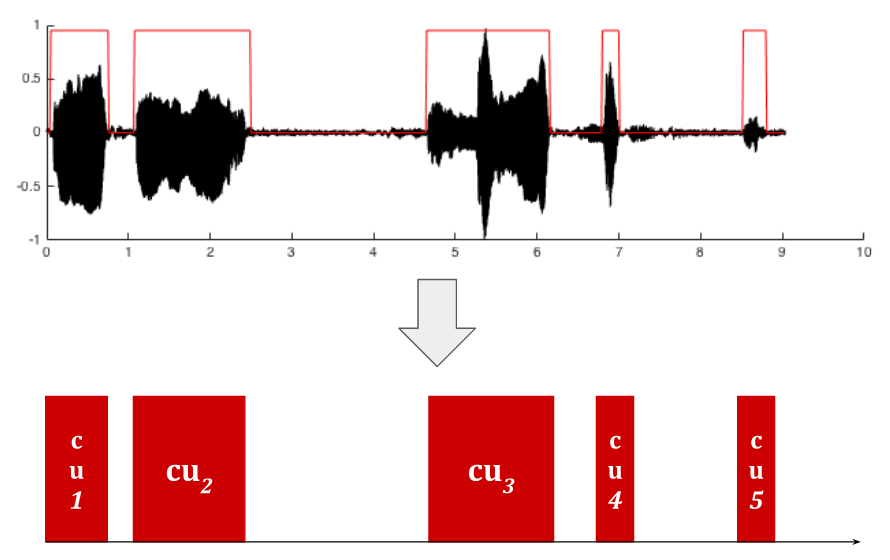
\includegraphics[width=0.6\textwidth]{bilder/vad_introduction02.png}
	\caption[Markierung stimmhafter Bereiche in einem Audiosignal]{Markierung stimmhafter Bereiche in einem Audiosignal. Oben Schwarz: Das Eingangssignal $x[\;]$. Oben Rot: Klassifizierung in \emph{stimmhaft}/\emph{nicht stimmhaft}. Unten Rot: Fünf erkannte Schreieinheiten $cu_1 , \ldots , cu_5$.}
	\label{img:vad01}
\end{figure}

In \autoref{sec:vad_new} wird die \emph{Voice Activity Detection} vorgestellt. In \autoref{sec:marking_cry-units_new} wird besprochen, wie stimmhafte Signalbereiche zu Schreieinheiten zusammengefasst werden. In \autoref{sec:decision_smoothing_new} wird ein Algorithmus vorgestellt, durch den inkorrekt erkannte Anfangs- und Endzeitpunkt von Schreieinheiten nachträglich korrigiert werden.

\section{Automatisierte Erkennung von Stimmaktivität in Signalen}
\label{sec:vad_new}

\emph{Voice Activity Detection} (kurz \emph{VAD}) oder \emph{Speech Detection}, die Feststellung des Vorhandenseins von Stimme in Signalbereichen, ist bei jeder Art der Sprachverarbeitung von Bedeutung: Im Mobilfunk wird sie beispielsweise eingesetzt, um die Zeitbereiche zu Erkennen, in denen Teilnehmer nicht sprechen und somit keine Übertragung stattfinden muss. Die größte Herausforderung von VAD-Systemen ist die robuste Erkennung von Stimmaktivität auch bei starkem Hintergrundrauschen. Bis heute wurde keine fehlerfreie Lösung für das Problem gefunden. \cite[S. 1]{vad_granada} \cite[S. 1]{vad_kola} \cite[S. 1]{vad_Lisboa}

Der Grundlegende Aufbau eines VAD-Algorithmus ist wie folgt. \autoref{img:vad_pipeline} visualisiert diesen Aufbau.
\begin{enumerate}
	\item \textbf{Vorverarbeitung} (engl. \emph{Pre-Proccessing}) des Signals.
	\item \textbf{Windowing: } Unterteilung des Signals in (einander überlappende) Signalfenster.
	\item \textbf{Extraktion von Eigenschaften} (engl. \emph{Feature-Extraction}) für jedes Signalfenster.
	\item \textbf{Entscheidung} (engl. \emph{Decision}) über die Präsens oder Abwesenheit von Stimme für jedes Signalfenster auf Grundlage der extrahierten Eigenschaften.
	\item \textbf{Entscheidungs-Glättung} (engl. \emph{Decision-Smoothing}), das nachträgliche Hinzufügen oder Entfernen von Entscheidungen mit Hilfe kontextueller Informationen der umliegenden Entscheidungen.\cite[S. 8 - 9]{vad_granada} \cite[S. 1 - 2]{vad_kola}
\end{enumerate}

\begin{figure}[h]
	\centering
	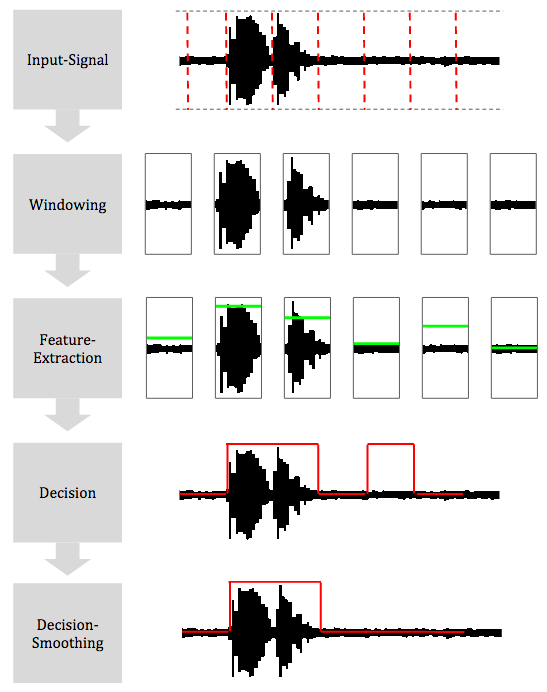
\includegraphics[width=0.6\textwidth]{bilder/vad_pipeline_04.png}
	\caption[Der grundlegende Aufbau eines VAD-Algorithmus]{Der grundlegende Aufbau eines VAD-Algorithmus (nach: \cite[S. 8]{vad_granada})}
	\label{img:vad_pipeline}
\end{figure}


In \autoref{sec:methods_vad_new} werden die Methoden vorgestellt, die zur Voice Activity Detection erprobt wurden. In \autoref{sec:vad_study} wird eine Simulationsstudie beschrieben, deren Ziel die Bestimmung derjenigen Methoden war, die sich für die VAD im speziellen Fall kindlicher Lautäußerungen am besten eignen. \autoref{sec:vad_results} fasst die Ergebnisse zusammen.

\subsection{Methoden}
\label{sec:methods_vad_new}

Die in diesem Unterabschnitt vorgestellten Methoden kombinieren Ideen, die von Moattar et al. \cite{vad_Easy}, Kristjansson et al. \cite{vad_Lisboa}, Waheed et al. \cite{vad_entropy}, Ahmadi et al. \cite{vad_ceps} und Shen et al. \cite{vad_entropie02} vorgestellt wurden.

\subsubsection{Einschränkung der zeitlichen Dynamik zur Vorverarbeitung}
\label{sec:preprocessing}

Bei der Vorverarbeitung werden Störeinflüsse auf das Signal minimiert, um die nachfolgenden Verarbeitungsschritte zu erleichtern. Welche Vorverarbeitung durchgeführt wird, ist abhängig von der konkreten Aufgabenstellung. Dieser Schritt ist für die VAD optional. So schlagen beispielsweise Ahmadi et al. \cite{vad_ceps} einen Bandpassfilter für die Vorverarbeitung vor, während Moattar et al. \cite{vad_Easy} keine Vorverarbeitung anwenden. 

In dieser Arbeit wurde sich für eine Vorverarbeitung entschieden, bei der das Signal hinsichtlich seiner Dynamik im Zeitbereich eingeschränkt wird. Dies ist ein typischer Vorverarbeitungsschritt bei Sprachaufnahmen. So wird vermieden, dass die durchschnittliche Energie des Signals für eine Erkennung der Stimmaktivität zu niedrig ist. Ein Grund für eine niedrige durchschnittliche Energie des Signals trotz maximaler Aussteuerung sind sehr kurze Pegelspitzen, deren Pegel weit über dem Durchschnittspegel liegen und so eine weitere Erhöhung der Lautstärke verhindern.\cite[S. 1 - 2]{schottland_comp}

Die Dynamikeinschränkung orientiert sich an der Arbeitsweise von Audiokompressoren. Dabei werden Signalspitzen, die über einen festgelegten \emph{Schwellwert} (engl. \emph{Threshold}) $\theta$ liegen, um ein festgelegtes \emph{Verhältnis} (engl. \emph{Ratio)} $\rho$ verringert. Ein Schwellwert von $\theta = 0.3$ mit einem Verhältnis von $\rho = 0.5$ bedeutet beispielsweise, dass alle Signalspitzen, die den Wert 0.3 über-, oder $-0.3$ unterschreiten, um 50\% verringert werden. Der Wert eines Samples nach der Kompression $x_{comp}[n]$ ergibt sich nach \autoref{eq:preprocessedX}.\cite[S. 400 - 401]{compressorPaper}

\begin{equation}
x_{comp}[n] =
\begin{cases}
\theta + (x[n] - \theta) \rho \quad , \text{wenn } x[n] > \theta \\
-\theta + (x[n] + \theta) \rho \quad, \text{wenn } x[n] < -\theta \\
x[n] \quad \text{sonst}
\end{cases}
\label{eq:preprocessedX}
\end{equation}

Die Amplituden hoher Signalspitzen werden so verringert und Headroom gewonnen, welcher anschließend bei der gleichmäßigen Erhöhung aller Amplituden zur Erhöhung der insgesamten Energie genutzt werden kann. \cite[S. 400 - 401]{compressorPaper}
    Diese Erhöhung kann beispielsweise durch eine Normalisierung nach \autoref{eq:normalizing} durchgeführt werden.

\begin{equation}
\text{normalize}(x_{comp}[n]) = \frac{x_{comp}[n]}{\maxi\{|x_{comp}[\;]|\}}
\label{eq:normalizing}
\end{equation}

In der Vorverarbeitung werden Threshold und Ratio nach \autoref{eq:THold} als Funktion des RMS-Wertes des Signals berechnet. Der Parameter $r_a$ gibt einen Ziel-RMS-Wert an.

\begin{equation}
\theta(x[\;]) = \rho(x[\;])  = \bigg[\frac{\text{RMS}(x[\;])}{r_a}\bigg]^{2}
\label{eq:THold}
\end{equation}

Die Vorverarbeitung eines Signals wird durchgeführt, indem 1.) die Kompression mit den Parametern nach \autoref{eq:preprocessedX} und 2.) die Normalisierung nach \autoref{eq:normalizing} durchgeführt wird. \autoref{img:compressing01} zeigt ein Signal vor und nach der Vorverarbeitung nach diesem Prinzip für $r_a = 0.18$ . Um eine zu große Beeinflussung des Signals zu vermeiden, wurde ein Minimalwert für Threshold und Ratio von $0.4$ festgelegt.

\begin{figure}[h]
	\centering
	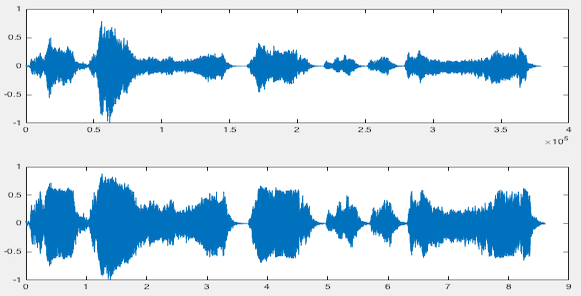
\includegraphics[width=0.6\textwidth]{bilder/compressing01.png}
	\caption[Vorverarbeitung der Voice Activity Detection]{Vorverarbeitung der Voice Activity Detection. Oben: Ein Beispielsignal vor der Vorverarbeitung. Unten: Das Beispielsignal nach der Vorverarbeitung.}
	\label{img:compressing01}
\end{figure}

Diese Vorverarbeitung eignet sich nicht für ein kontinuierliches System, da zur Berechnung des RMS-Wertes alle Samples des Signals bereits bekannt sein müssen. Das Hauptziel dieser Vorverarbeitung war die Gewährleistung ähnlicher Energieverhältnisse bei den Signalen des Trainingsdatensatzes, die in der Simulationsstudie in \autoref{sec:vad_study} verwendet wurden. Dabei wurde $r_a = 1.8$ festgelegt. Das folgende Vorgehen für den Einsatz dieser Vorverarbeitung in einem kontinuierlichen System wird vorgeschlagen:
\begin{itemize}
	\item Komplettes Überspringen der Vorverarbeitung, indem mit Hilfe eines manuell einstellbaren Lautstärkereglers eine ausreichende Signalenergie gewährleistet wird. Würde man beispielsweise anstelle der Analyse des Audiosignals ein Videosignal zur Schmerzbewertung des Gesichtsausdrucks verwenden, wäre eine Ausreichende Bildhelligkeit eine Voraussetzung für die Bilderkennung.
	\item Die Initialisierung des Kompressor mit \grqq sanften Werten\grqq , wie zum Beispiel $\theta = \rho = 0.7$. Diese Parameter können nach der Beendigung eines Schrei-Segmentes (siehe \autoref{sec:segmenting}) auf Basis des RMS-Wertes des Segmentes aktualisiert und für die Vorverarbeitung der darauf folgenden Signalbereiche eingesetzt werden.
\end{itemize}

\subsubsection{Zerlegung des Signals in überlappende Fenster}
\label{sec:windowing}

Angenommen, man führt die Voice Activity Detection für das Signal $x[\;]$ durch und kommt zu dem Schluss, dass in dem Signal (teilweise) Stimme enthalten ist. Ist das Signal mehrere Minuten oder sogar Stunden lang, ist allein aus diesem Schluss nicht ersichtlich, in welchen Zeitbereichen des Signals Stimme enthalten ist, und in welchen nicht. Um die zeitliche Auflösung zu erhöhen, wird das Signal in kürzere Zeitfenster zerlegt.

Nach der Vorverarbeitung wird diese Zerlegung mit Hilfe der in \autoref{sec:stft} als \emph{Windowing} bezeichneten Methode durchgeführt. Das Signal $x[\;]$ wird nach \autoref{eq:signal-Window} in die Signalfenster $x_0[\;] , \ldots , x_m[\;]$ aufgeteilt. Die Zeitfenster werden zunächst im Zeitbereich belassen. Es wurde sich für die von Waheed et al. \cite{vad_entropy} vorgeschlagene Fensterlänge von \SI{25}{\milli\second} entschieden, als Kompromiss zwischen den von Moattar et al. \cite{vad_Easy} empfohlenen \SI{10}{\milli\second} und den von Ahmadi et al. \cite{vad_ceps} empfohlenen \SI{40}{\milli\second}. Die Fenster überlappen einander um 50\%, das heißt \SI{12.5}{\milli\second}.

Die Entscheidung über das Vorhandensein von Stimme wird \emph{einzeln} für jedes der Signalfenster $x_0[\;] , \ldots , x_m[\;]$ durchgeführt. Grundlage für die Entscheidung ist eine Menge an Attributen, die für das jeweilige Signalfenster $x_i[\;]$ berechnet wird. Die Ermittlung und Evaluation geeigneter Attribute ist einer der primären Forschungsbereiche in der VAD. In den folgenden Unterabschnitten \ref{sec:vad_time_features} bis \ref{sec:vad_dif_feature} wird eine Reihe an Features vorgestellt, die in dieser Arbeit zur VAD erprobt wurden. Jedes der in diesen Unterabschnitten besprochenen Features kann für ein Signalfenster $x_i[\;]$ \`{a} \SI{25}{\milli\second} berechnet werden und als Grundlage für eine Entscheidung dienen. Die Evaluation dessen, welche Attribute sich am besten als Entscheidungsgrundlage zur Feststellung von Babylauten eignen, folgt in \autoref{sec:vad_study}. Die Ergebnisse werden in \autoref{sec:vad_results} zusammengefasst.

\subsubsection{Eigenschaften des Zeitbereiches}
\label{sec:vad_time_features}

Im Zeitbereich wurden die beiden Eigenschaften \emph{Root Mean Square} [\emph{RMS}] und \emph{Zero Crossing Rate} [\emph{ZCR}] erprobt.

Moattar et al. \cite[S. 2549]{vad_Easy} bezeichnen den Energiegehalt eines Signals als das für die VAD am häufigsten angewandte Attribut. Der RMS-Wert als Feature für ein Signalfenster wird nach \autoref{eq:rms} berechnet. Hintergrund ist, dass der Energiegehalt eines Stimmsignals typischerweise höher ist als der des Hintergrundrauschens. Bei geringem Signal-Rausch-Abständen ist diese Bedingung jedoch nicht immer erfüllt. Als zweites Attribut des Zeitbereiches wurde die \emph{Zero Crossing Rate} nach \autoref{eq:zcr} berechnet. Dieses Feature misst die Häufigkeit eines Vorzeichenwechsels im Signal. Stimmlose Signalbereiche haben typischerweise eine höhere ZCR als stimmhafte Signalbereiche. Problematisch ist dieses Kriterium bei Signalen, bei denen kein Hintergrundrauschen vorliegt, da sich dort eine ZCR von 0 ergibt.\cite[S. 335 - 336]{vad_ceps} Um den Wert in Relation zur Fensterlänge setzen zu können, wird die ZCR durch die Anzahl der Samples eines Signalfensters $N$ geteilt.

\begin{equation}
\text{ZCR}(x_i[\;]) = \sum_{0}^{N-1}|\text{sng}(x_i[n])-\text{sng}(x_i[n-1])|
\label{eq:zcr}
\end{equation}

\subsubsection{Eigenschaften der Autokorrelation}

Neben dem RMS-Wert und der ZCR wurde die Autokorrelation zur VAD erprobt. Die Autokorrelation eignet sich, um Periodizität in einem Signal nachzuweisen. Wie in \autoref{sec:theVoice} erläutert wurde, weisen stimmhafte Signale ein tendenziell stärker periodisches Verhalten als stimmlose Signalteile auf. 

Bei der Autokorrelation wird ein Signal mit einer verzögerten Variante von sich selbst korreliert. \autoref{eq:ACorr} definiert die Autokorrelation des $N$-Sample langen Signalfensters $x_i[\;]$, verzögert um einen als \emph{Lag} bezeichneten Wert $k$.\cite[S. 1]{vad_Lisboa}

\begin{equation}
\text{A-Corr}_k(x[\;]) = \sum_{n=k}^{N} x[n-k] \cdot x[n]
\label{eq:ACorr}
\end{equation}

Da der Autokorrelationswert neben der Stärke der Periodizität von der Signalenergie abhängig ist, ist eine Normalisierung des Wertes wünschenswert. Es gibt verschiedene Varianten dieser Normalisierung. \autoref{eq:NACorr} definiert die \glqq normalisierte Autokorrelation\grqq{}, bei der der Autokorrelationswert durch die RMS-Werte des verzögerten und des unverzögerten Signals normalisiert wird. Ein hoher Wert der normalisierten Autokorrelation mit der Verzögerung $k$ spricht für eine ausgeprägte Periodizität des Signals mit der Frequenz $f =  f_s / k $.\cite[S. 1 - 2]{vad_Lisboa}

\begin{equation}
\text{NA-Corr}_k(x[\;]) = \frac{\sum_{n=k}^{N} x[n-k] \cdot x[n]}{ \sqrt{\sum_{n=1}^{N-k}  x[n]^2}  \cdot  \sqrt{\sum_{n=k}^{N}  x[n]^2} }
\label{eq:NACorr}
\end{equation}

%Das Autokorrelations-Signal $a[\;]$ wird erstellt, indem die normalisierte Autokorrelation für verschiedene $k = k_{min} , \ldots , k_{max}$ angewandt wird, wie Gleichung \ref{eq:a-Signal} definiert. 

%\begin{equation}
%a[\;] := \quad \mathop{\forall}_{k = k_{min}}^{k_{max}} :\ a[k] = \text{NA-Corr}_k(x[\;]) 
%\label{eq:a-Signal}
%\end{equation}

In Bezug auf die VAD wurde die Autokorrelation als Methode genutzt, um die beiden Attribute \emph{höchste Autokorrelationsspitze} [\emph{aMax}] und \emph{Anzahl der Autokorrelationsspitzen} [\emph{aCount}] zu berechnen. Beide Eigenschaften wurden von Kristjansson et al. \cite[S. 1 - 2]{vad_Lisboa} zur VAD beschrieben. Die \emph{höchste Autokorrelationsspitze} wird in \autoref{eq:corrpeak} definiert und bestimmt die höchste Magnitude der normalisierten Autokorrelation für die Verzögerungswerte $k_{min} , \ldots , k_{max}$. Ein stimmhaftes Signal hat aufgrund seiner Periodizität erwartungsgemäß einen höheren [\emph{aMax}]-Wert als Rauschen.

\begin{equation}
\text{aMax}(x_i[\;]) = \maxmagi_{k = k_{min} \: \ldots \: k_{max}}\{\text{NA-Corr}_k(x_i[\;])\}
\label{eq:corrpeak}
\end{equation}

Die \emph{Anzahl der Autokorrelationsspitzen} wird nach \autoref{eq:corrcount} berechnet. Das Feature gibt an, wie viele Signalspitzen im Autokorrelationssignal enthalten sind. Rauschen erzeugt höhere [\emph{aCount}]-Werte als stimmhafte Signale, bedingt durch die vielen zufällig verteilten Periodizitäten.\cite[S. 1 - 2]{vad_Lisboa}

\begin{equation}
\text{aCount}(x_i[\;]) = \counti_{k = k_{min} \: \ldots \: k_{max}}\{\text{NA-Corr}_k(x_i[\;])\}
\label{eq:corrcount}
\end{equation}

Das Verzögerungsintervall $k_{min} , \ldots , k_{max}$ wurde so gewählt, dass Periodizitäten nur in dem Bereich gesucht wurden, der für die Grundfrequenz von Babystimmen in Frage kommt. Aus \autoref{sec:acousticModel} ging hervor, dass diese Grundfrequenz für Babys zwischen $250$ und $\SI{2000}{\hertz}$ liegt.

\subsubsection{Eigenschaften des Frequenzbereiches}

auf Basis des Frequenzbereiches wurden die drei Eigenschaften \emph{unnormalisierte spektrale Entropie} [$SEnt_{u}$], \emph{normalisierte spektrale Entropie}  [$SEnt_{n}$] und \emph{dominanteste Frequenzkomponenten} [$f_{dom}$] erprobt.\cite{vad_Lisboa}

Als Vorbereitungsschritt wird das Signalfenster des Zeitbereiches $x_i[\;]$ in den Frequenzbereich $X_i[\;]$ transformiert. Die Berechnungsvorschrift ist $X_i[\;] = \text{DFT}\{(w[\;] \cdot x_i[\;])\}$. Wird diese Transformation für alle Signalfenster $x_0[\;], \ldots, x_m[\;]$ durchgeführt, entspricht dies der in \autoref{sec:stft} vorgestellten Kurzzeit-Fourier-Transformation des ursprünglichen Eingangssignals $x[\;]$. Es wurde eine $2048$ Punkte lange FFT und ein Hamming-Window als Fensterfunktion $w[\;]$ verwendet.

Kristjansson et al. \cite[S. 2]{vad_Lisboa} haben die \emph{spektrale Entropie} zur VAD beschrieben. Dabei wird das Spektrum des Frequenzfensters $X_i[\;]$ als Wahrscheinlichkeitsverteilung betrachtet. Die Entropie als Maß zur \glqq Unreinheit\grqq{} wurde in \autoref{sec:id3} erläutert. Die \emph{normalisierte spektrale Entropie} wird nach der \autoref{eq:norm_se} berechnet. Das Signal $px_i[\;]$ ergibt sich durch die Normalisierung des $N$-Punkte langen Spektrums nach \autoref{eq:norm_spek}. Bei der normalisierten spektralen Entropie ist zu erwarten, dass Frequenzfenster ohne Stimme einen höheren Wert aufweisen als Fenster mit Stimme.\cite[S. 2]{vad_Lisboa} 

\begin{equation}
px_i[n] = \frac{X_i[n]}{\sum_{k=1}^{N} X_i[k]}
\label{eq:norm_spek}
\end{equation}

\begin{equation}
\text{SEnt}_n(px_i[\;]) = -\sum_{k=1}^{N}px_i[k] \cdot\log(px_i[k])
\label{eq:norm_se}
\end{equation}

Neben der von Kristjansson et al. \cite{vad_Lisboa} vorgestellten normalisierten spektralen Entropie wurde zusätzlich die \emph{unnormalisierte Spektrale Entropie} nach \autoref{eq:unnnorm_se} berechnet. Bei dieser wird das Spektrum nicht normalisiert, das heißt, es gilt $px_i[k] = X_i[k]$. Somit hat die Energie des Signals einen größeren Einfluss auf den Wert des Attributes. Dabei ist zu erwarten, dass Signalfenster mit Stimme einen höheren Wert aufweisen als solche mit Rauschen.

%\footnote{Kristjansson et al \cite[S. 2]{vad_Lisboa} verwenden zur Entropie-Berechnung den Logarithmus zur Basis 10, anstatt zur Basis 2. Es ist nicht klar, ob es sich dabei um einen Fehler handelt. In dieser Arbeit wurde, wie in der Publikation beschrieben, ebenfalls der Logarithmus zur Basis 10 verwendet.}

\begin{equation}
\text{SEnt}_u(X_i[\;]) = -\sum_{k=1}^{N}X_i[k] \cdot\log(X_i[k])
\label{eq:unnnorm_se}
\end{equation}

In die Berechnungen wurden nur die Frequenzen im Bereich von 250 - \SI{8000}{\hertz} mit einbezogen, da nach \autoref{sec:acousticModel} die tiefst mögliche Grundfrequenz einer Babystimme bei \SI{250}{\hertz} liegt und nach Shen et al. \cite{vad_entropie02} die Stimme keine Informationen oberhalb von \SI{8000}{\hertz} enthält.

Moattar et al. \cite[S. 2550]{vad_Easy} haben die \emph{dominanteste Frequenzkomponente} zur VAD vorgestellt. Für jedes Frequenzfenster $X_i[\;]$ wird diejenige Frequenz nach  \autoref{eq:domfreq} berechnet, welche die höchste Amplitude hat. Es wird dabei, im Gegensatz zur spektralen Entropie, der gesamte Frequenzraum betrachtet. Ein stimmhaftes Signal hat typischerweise eine höhere $f_{dom}$ als ein stimmloses Signal, bedingt durch die hohe Amplitude der Grundfrequenz.\cite[S. 2550]{vad_Easy}

\begin{equation}
f_{dom}(X_i[\;]) = \argmax \{X_i[\;]\}
\label{eq:domfreq}
\end{equation}


\subsubsection{Eigenschaften des Cepstrums}
\label{sec:vad_ceps_features}

Das Cepstrum wird nach \autoref{eq:cepstrum} als die inverse DFT des Logarithmus des Magnitudensignals des Frequenzbereiches definiert.\cite[\emph{Cepstral Analysis}, S. 2]{ricardo_ceps}

\begin{equation}
c[\;] =  \text{iDFT}\Big\{ \log \Big(\ \big|\ \text{DFT}\{x[\;]\} \big|\ \Big) \Big\}
\label{eq:cepstrum}
\end{equation}	

\begin{figure}[h]
	\centering
	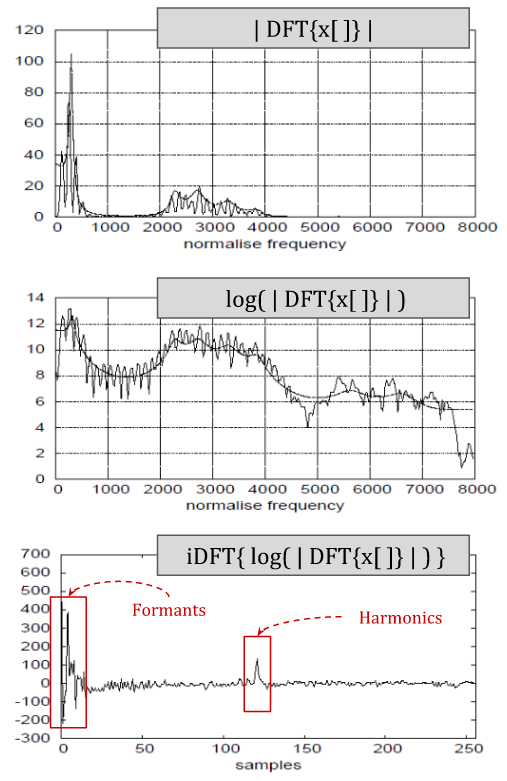
\includegraphics[width=0.55\textwidth]{bilder/cepstrum04.png}
	\caption[Berechnung des Cepstrums]{Berechnung des Cepstrums. (nach: \cite[\emph{Cepstral Analysis}, S. 3]{ricardo_ceps})}
	\label{img:cepstrumOverview}
\end{figure}

Das Vorgehen wird mit Hilfe des Beispiels aus \autoref{img:cepstrumOverview} erläutert. $ |\ \text{DFT}\{x[\;]\}\ \big| $  zeigt das Spektrum eines \glqq typischen stimmhaften\grqq{} Signals $x[\;]$. Es sind die in \autoref{sec:theVoice} erläuterten, für ein stimmhaftes Signal typischen harmonischen Obertöne zu sehen, welche mit steigender Frequenz an Amplitude verlieren. Durch das Logarithmieren des Spektrums $\log \big(\ |\ \text{DFT}\{x[\;]\} |\ \big)$ wird die Dynamik des Frequenzbereiches verringert und somit der Amplitudenverlust der höheren Obertöne reduziert. Man stelle sich vor, dieses Spektrum wäre ein Signal des Zeitbereiches. In diesem Fall würde man die harmonischen Obertöne als ein annähernd periodisches Signal betrachten, welches von einem niederfrequenten Signal überlagert wird. Um diese beiden Frequenzkomponenten voneinander zu trennen, müsste man eine weitere DFT anwenden. Diese DFT kommt in dem Fall einer inversen DFT gleich, da das Phasen-Signal verworfen wurde. Man erwartet in diesem \glqq Spektrum vom Spektrum\grqq{} eine Signalspitze im \glqq oberen Frequenzbereich\grqq , bedingt durch die harmonischen Obertöne, sowie eine Signalspitze im \glqq unteren Frequenzbereich\grqq, bedingt durch die Formanten.\cite[\emph{Cepstral analysis}, S. 4]{ricardo_ceps}

Der Bereich dieser \glqq Fourier-Transformation der Fourier-Transformation\grqq{} wird als \emph{Cepstrum} bezeichnet. Cepstrum ist ein ein Wortspiel, welches durch die Umkehrung der ersten vier Buchstaben des Wortes \glqq Spectrum\grqq{} entsteht. Die unabhängige Variable des Cepstrum wird als \emph{Quefrency} bezeichnet. So wird verdeutlicht, dass die unabhängige Variable dieses Bereichs zwar mathematisch betrachtet die Zeit darstellt, jedoch als Frequenz interpretiert wird.\cite[\emph{Cepstral analysis}, S. 7]{ricardo_ceps}	

Ein Aufkommen einer Signalspitze im oberen Quefrency-Bereich $> \SI{3}{\milli\second}$ spricht für das Vorhandensein von harmonischen Obertönen im Signal, wie sie beispielsweise durch Stimme erzeugt werden. \autoref{img:cepstrumVoicedPeak} verdeutlicht das Prinzip an einem Beispiel. Zu sehen ist die Kurzzeit-Fourier-Transformation eines Signals mit einer Fensterlänge von $\SI{50}{\milli\second}$ und einer Hopsize von $\SI{12.5}{\milli\second}$. Links wird das logarithmierte Spektrum des entsprechenden Frequenzfensters abgebildet, rechts das Cepstrum. Die Frames 1 bis 5 sind stimmlos und die Frames 8 bis 15 sind stimmhaft. Die Frames 6 und 7 bilden eine Zwischenform zwischen stimmhaft und nicht-stimmhaft. Wie zu sehen ist, haben die Cepstren der stimmhaften Frames eine Signalspitze bei der Quefrency $q \approx \SI{12}{\milli\second}$.\cite[\emph{Cepstral Analysis}, S. 16]{ricardo_ceps}

\begin{figure}[h]
	\centering
	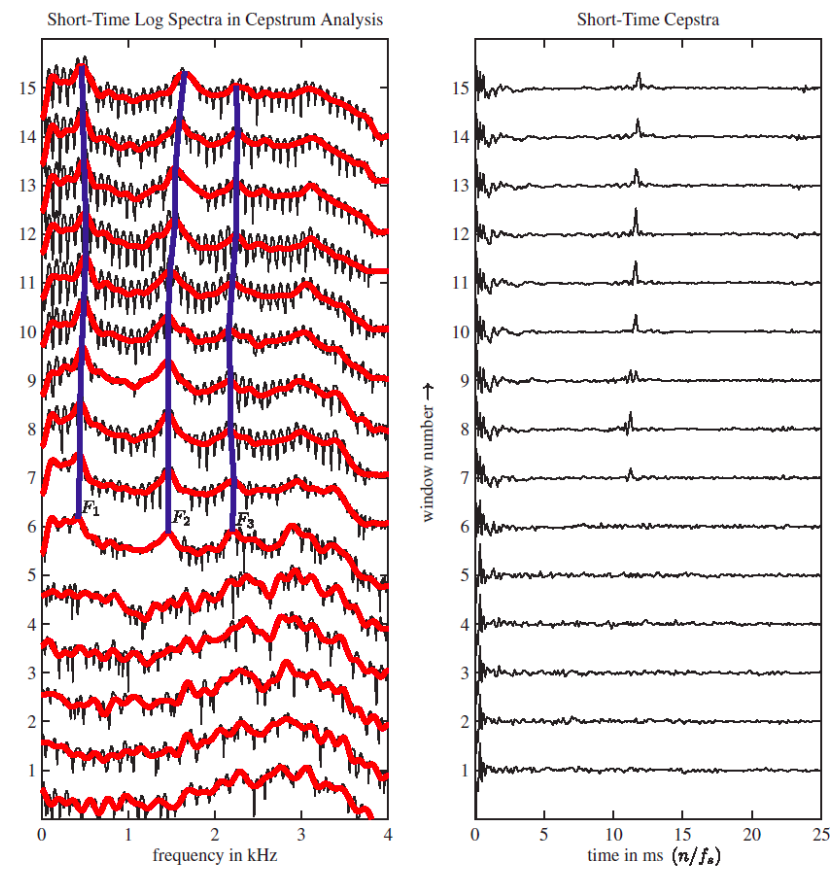
\includegraphics[width=0.6\textwidth]{bilder/cepstrum05.png}
	\caption[Aufkommen einer Signalspitze im oberen Quefrency-Bereich]{Aufkommen einer Signalspitze im oberen Quefrency-Bereich bei stimmhaften Signalfenstern. \cite[\emph{Cepstral Analysis}, S. 17]{ricardo_ceps}}
	\label{img:cepstrumVoicedPeak}
\end{figure}

\autoref{img:cepstrumPitch} verdeutlicht, wie eine Periode von $T_0$ im Zeitbereich eine Signalspitze im Frequenzbereich bei der Grundfrequenz $f_0$ bedingt, welche wiederum in Verbindung mit den harmonischen Obertönen eine Signalspitze bei der Quefrency $q_o = 1 / f_0$ im Cepstrum verursacht. Wird somit in einem Cepstrum eine Signalspitze bei $q_0$ festgestellt, weißt dies auf eine Grundfrequenz von $f_0 = 1/q_0$ hin. \cite[S. 5]{cepstrumPitchTranslation}

In Bezug auf die VAD wurde das Cepstrum genutzt, um die beiden Features \emph{Höchster Peak im Cepstrum} [$Ceps_{mag}$] und \emph{Quefrency des höchsten Peaks} [$Ceps_{loc}$] zu berechnen.

Ahmadi et al. \cite{vad_ceps} sowie Kristjansson et al. \cite{vad_Lisboa} schlugen vor, die Magnitude der höchsten Signalspitze im oberen Bereich des Cepstrums als Maß für die Stimmhaftigkeit eines Signals einzusetzen. \autoref{eq:ceps_maxpeak} definiert die Berechnung dieses Attributs. $c_i[\;]$ ist das Cepstrum des $i$-ten Frequenzfensters $X_i[\;]$. So wie bei den Attributen der Autokorrelation wurde, entsprechend den möglichen Grundfrequenzen von Babystimmen, ein Quefrency-Bereich von $q_{min} = 5$ bis $q_{max} = \SI{40}{\milli\second}$ durchsucht.

\begin{equation}
Ceps_{mag}(c_i[\;]) = \maxmagi_{q = q_{min} \ldots , q_{max}}\{ \; c_i[q] \; \}
\label{eq:ceps_maxpeak}
\end{equation}

Als zweites Attribut, welches auf dem Cepstrum basiert, wurde die Quefrency der höchsten Amplitude des oberen Quefrency-Bereiches nach \autoref{eq:ceps_loc} berechnet. Bei Signalfenstern ohne Stimme ist es wahrscheinlicher, dass sich die höchste Amplitude am Mindest- oder Maximalwert des durchsuchten Quefrency-Bereiches befindet.

\begin{equation}
Ceps_{loc}(c_i[\;]) = \argmax_{q = q_{min} \ldots , q_{max}} \{ \; c_i[q] \; \}
\label{eq:ceps_loc}
\end{equation}	

\begin{figure}[h]
	\centering
	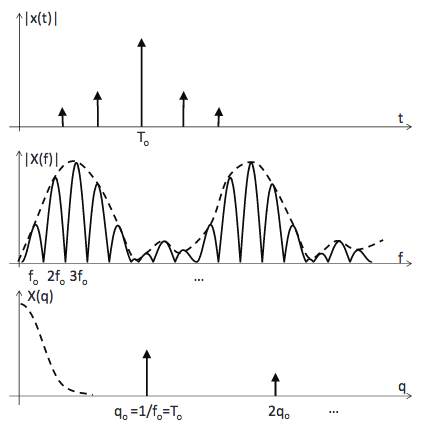
\includegraphics[width=0.5\textwidth]{bilder/cepstrumPitch.png}
	\caption[Feststellung der Grundfrequenz aus dem Cepstrum]{Feststellung der Grundfrequenz aus dem Cepstrum \cite[S. 5]{cepstrumPitchTranslation}}
	\label{img:cepstrumPitch}
\end{figure}

\subsubsection{Differenz-Features}
\label{sec:vad_dif_feature}

\autoref{img:vadAllFeatures} visualisiert alle Attribute, die in den vorangegangenen Unterabschnitten zur VAD vorgestellt wurden. Der oberste Plot zeigt das Audiosignal aus \autoref{img:vad01} mit einem Signal-Rausch-Abstand von \SI{20}{\decibel}. Die rote Linie des obersten Plots klassifiziert die Zeitbereiche in $1 \; \hat{=} $ \emph{stimmhaft} und $0 \; \hat{=}$ \emph{nicht stimmhaft}. Alle darunter liegenden Plots zeigen den zeitlichen Verlauf der entsprechenden Attribute.

\autoref{img:min-signal} zeigt den zeitlichen Verlauf des RMS-Features im Detail. (A) zeigt das verhalten des \emph{RMS}-Attributes bei einem Signal-Rausch-Abstand von \SI{50}{\decibel}. Die stimmlosen Zeiträume haben einen weitaus niedrigeren RMS-Wert als die Zeiträume mit Stimme. In (B) ist das selbe Signal mit einem Signal-Rausch-Abstand von \SI{3}{\decibel} zu sehen. Nun liegen die RMS-Werte der stimmlosen Bereiche nur noch knapp unter denen des Sprachsignals. Zu sehen ist, dass starkes Hintergrundrauschen ähnlich hohe Feature-Werte erzeugen kann wie die Stimme.

\begin{figure}[H]
	\centering
	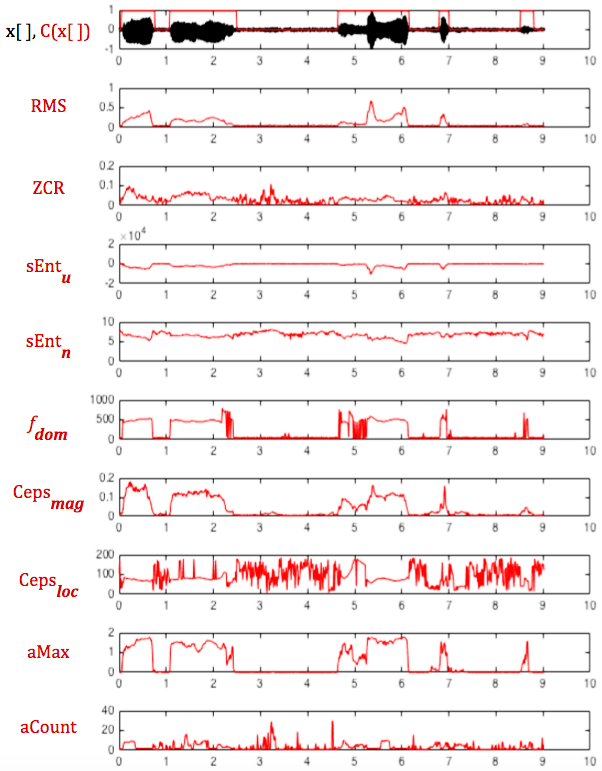
\includegraphics[width=0.85\textwidth]{bilder/allFeatures03.png}
	\caption[Übersicht über alle Attribute, die für die VAD erprobt wurden]{Übersicht über alle Attribute, die für die Voice Activity Detection erprobt wurden.}
	\label{img:vadAllFeatures}
\end{figure}

Moattar et al. \cite{vad_Easy} und Waheed et al. \cite{vad_entropy} schlugen vor, den Wert des jeweiligen Attributes zu messen, der in den stimmlosen Bereichen durch das Hintergrundrauschen erzeugt wird. Es kann davon ausgegangen werden, dass die ersten Signalfenster eines Signals stimmlos sind, und der Feature-Wert des Rauschens somit anhand dieser Fenster bestimmt werden kann. Bei einer langanhaltenden und kontinuierlichen Analyse können sich sowohl der Signal-Rausch-Abstand als auch die Qualität des Rauschens ständig ändern, weshalb in von den stimmlosen Bereichen erzeugten Attributwerte regelmäßig aktualisiert werden müssen. Es kann weiterhin davon ausgegangen werden, dass die Länge einer Cry-Unit eine bestimmte Länge $t_{max}$ nicht überschreiten kann, bevor das Baby Luft holen muss und somit mindestens ein stimmloses Zeitfenster entsteht, welches das Hintergrundrauschen enthält. Zeskind et al. \cite[S. 325]{rythmic} haben $t_{max} = \SI{4.75}{\second}$ bestimmt. In einem Zeitbereich $ t > t_{max}$ muss somit zumindest ein Feature-Wert enthalten sein, der durch stimmlose Singalbereiche erzeugt wurde. 

\begin{figure}[h]
	\centering
	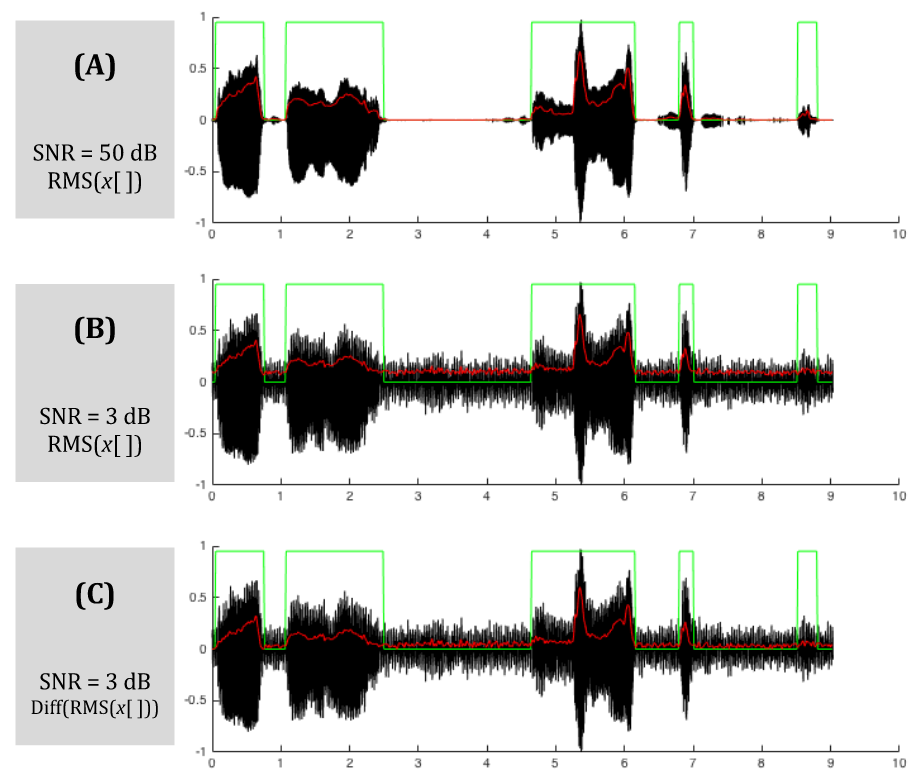
\includegraphics[width=0.7\textwidth]{bilder/rms_diff.png}
	\caption[Das RMS-Feature bei verschiedenen Signal-Rausch-Abständen]{Das RMS-Feature bei verschiedenen Signal-Rausch-Abständen. Schwarz: Eingangs-Signal $x[\;]$. Grün: Klassifizierung in \emph{stimmhaft/nicht stimmhaft}. Rot: zeitlicher Verlauf des RMS-Features.}
	\label{img:min-signal}
\end{figure}

Auf Basis dieser Überlegung wurde das \emph{Differenz-Feature} Diff\textsubscript{t}(Feat$(x_i[\;])$) nach \autoref{eq:difFeature} definiert als die Differenz zwischen einem aktuell gemessenen Attributwerte und dem geringsten Attributwerte, welcher im vergangenen Zeitbereich $t$ gemessen wurde. Feat$(x_i[\;])$ bezeichnet dabei einen beliebigen Feature-Wert des Signalfensters $x_i[\;]$, $t_{xi}$ die Länge eines Signalfensters in Sekunden (in diesem Fall \SI{25}{\milli\second}), und $t$ den zu durchsuchende Zeitbereich in Sekunden $> t_{max}$, welcher von dem jeweiligen Signalfenster $x[\;]$ aus betrachtet in der Vergangenheit liegt. In \autoref{img:min-signal} wird in (C) das Differenz-Feature für den RMS-Wertes gezeigt.

\begin{equation}
\text{Diff}_t(\text{Feat}(x_i[\;])) = \text{Feat}(x_i[\;])\ - \mini_{k=(i-z)...i}\{\text{Feat}(x_k[\;])\} \qquad , z = \frac{2 \cdot t}{t_{xi}}
\label{eq:difFeature}
\end{equation}

In dieser Arbeit wurde $t = \SI{5}{\second}$ festgelegt. Es ist zu beachten, dass die Attribute \emph{ZCR, SEnt\textsubscript{u}} und \emph{aCount} zur Berechnung des Differenz-Features bezüglich ihres Vorzeichens invertiert werden müssen, da bei ihnen niedrige an Stelle hoher Werte stimmhafte Signale anzeigen. Das einzige Attribut, für dass die Berechnung des Differenz-Features keinen Sinn macht, ist das \emph{Ceps\textsubscript{loc}}-Attribut, da es bei stimmlosen Signalabschnitten sowohl einen höheren als auch einen niedrigeren Wert annehmen kann.

\subsubsection{Entscheidung über das Vorhandensein von Stimme auf Basis der Attribute}

Eine einfache Variante zur Entscheidung darüber, ob ein Signalfenster $x_i[\;]$ Stimme enthält, ist, eines der vorgestellten Attribute als Entscheidungsgrundlage zu wählen und einen festen Grenzwert $\theta$ festzulegen, bei dessen Über- oder Unterschreitung das Fenster als stimmhaft klassifiziert wird. Die Entscheidung lässt sich als \emph{Klassifizierungsfunktion} (auch: \emph{Klassifikator}) $C: \{ x_i[\;] \} \mapsto Y$ definieren, welche ein Signalfenster abbildet auf $Y = \{ 1 \; \hat{=} \; \text{stimmhaft}, \; 0 \; \hat{=} \; \text{nicht stimmhaft}\}$. Die Klassifizierungsfunktion nimmt dann die folgende Form an:

\begin{equation}
	C(x_i[\;]) = 
\begin{cases}
1 \quad , \text{wenn Feat}(x_i[\;]) > \theta \\
0 \quad , \text{sonst}
 \end{cases}
\end{equation}

\autoref{img:thresholded} verdeutlicht das Prinzip an einem Beispiel. Das Feature, dass als Entscheidungsgrundlage genutzt wird, ist der \emph{RMS}-Wert. Ein Grenzwert von $\theta = 0.18$ gewährleistet in diesem Fall eine weitestgehend richtige Klassifizierung.

\begin{figure}[h]
	\centering
	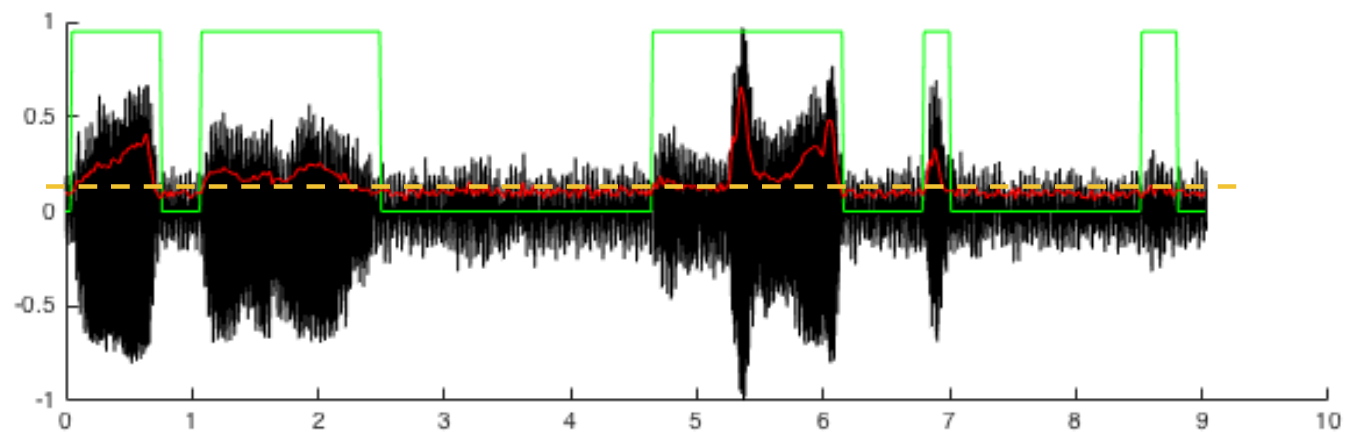
\includegraphics[width=0.65\textwidth]{bilder/thresholded02.png}
	\caption[Beispiel für die Grenzwertsetzung eines Features]{Beispiel für die Grenzwertsetzung eines Features. Schwarz: Das Eingangssignal $x[\;]$. Grün: Klassifizierung in \emph{stimmhaft/nicht stimmhaft}. Rot: RMS-Feature. Gelb: Grenzwert}
	\label{img:thresholded}
\end{figure}

Es stellt sich die Frage, wie man für ein Attribut einen Grenzwert findet, der für verschiede Signal-Rausch-Abstände eine möglichst hohe Klassifikationsgenauigkeit gewährleistet. In einigen Veröffentlichungen, so wie der von Moattar et al. \cite{vad_Easy}, wird empfohlen, den Grenzwert experimentell festzustellen. In dieser Arbeit wurde sich für den Ansatz einer automatisierten, datengetriebenen Grenzwertsuche mit Hilfe des in \autoref{sec:id3} vorgestellten \emph{C4.5}-Algorithmus entschieden. Der Grundgedanke ist wie folgt: Angenommen, man hat eine Datenbank zur Verfügung, bestehend aus einer Menge an Signalen mit Audioaufnahmen kindlicher Lautäußerungen, in denen manuell die stimmhaften Signalabschnitte markiert wurden. Diese Signale zerlegt man nach den vorgestellten Methoden in kürzere Signalfenster und berechnet für jedes Signalfenster das Feature, dessen Grenzwert man sucht. Jedes Signalfenster versieht man außerdem mit dem Klassenlabel $y \in Y$ auf Basis der manuellen Markierungen. Ein \emph{Signalfenster} $x_i[\;]$ wird so zu einem \emph{Exempel} $e_i = (\text{Feat}(x_i[\;]), y_i)$. Alle Exempel werden zu einem \emph{Trainingsdatensatz} zusammengetragen. Nun kann der \emph{C4.5}-Algorithmus verwendet werden, um für das Feature den Grenzwert zu finden, der für diesen Datensatz die Klassifizierung mit der höchsten Genauigkeit vornimmt. Voraussetzung dafür ist, dass die maximale Tiefe des zur Klassifizierung entworfenen Entscheidungsbaums mit 1 bestimmt wird, damit für das jeweilige Attribut genau ein Grenzwert festgelegt wird. Ist das Attribut, für das der Grenzwert gesucht wird, ein Differenz-Feature, so lässt sich der Grenzwert als ein adaptiver Grenzwert interpretieren, der sich an den aktuellen SNR anpasst.

%besser formulieren!
Die Verwendung des \emph{C4.5}-Algorithmus bringt die Möglichkeit mit sich, eine beliebige Menge an Features in die Klassifizierung mit einzubeziehen. Die Klassifizierung muss also nicht zwingend auf Grundlage nur eines Attributes geschehen. Angenommen, es werden die beiden Features $RMS$ und $ZCR$ für jedes Signalfenster einer Datenbank berechnet, dann enthält jedes Exempel des so konstruierten Trainingsdatensatzes diese beiden Features. Wird dieser Trainingsdatensatz dem \emph{C4.5}-Algorithmus zum Entwurf eines Klassifikators gegeben, dann nimmt der Klassifikator die Form eines Entscheidungsbaumes an, bei dem durch das hierarchische Setzen von Grenzwerten die Klassifizierung vorgenommen wird. \autoref{lst:tree01} zeigt ein Beispiel für eine so resultierenden, fiktiven Klassifikator.

\begin{lstlisting}[frame=single,mathescape=true,basicstyle=\footnotesize,language=Java,label=lst:tree01,caption=Beispiel eines Entscheidungsbaums für die Klassifizierung bei der VAD,linewidth=1\textwidth]
if RMS($x_i[\;]$) > 0.2
|   if ZCR($x_i[\;]$) < 0.13
|   |   C($x_i[\;]$) = 0
|   |else
|   |   C($x_i[\;]$) = 1
|else
|    C($x_i[\;]$) = 1
\end{lstlisting}

Wird dem \emph{C4.5}-Algorithmus eine größere Menge an Attributen zur Verfügung gestellt, auf deren Basis der Klassifikator entworfen wird, wird der Entscheidungsbaum implizit zeigen, welche Features für die VAD besser geeignet sind, da sie höher im Entscheidungsbaum erscheinen. Es besteht jedoch die Gefahr, dass der Algorithmus in ein lokales Maximum gelaufen ist und der entworfene Klassifikator somit eine suboptimale Auswahl an Features verwendet. Außerdem besteht die Gefahr des Overfitting, insofern Entscheidungsbäume mit beliebiger Tiefe zugelassen werden.

\subsection{Simulationsstudie zur Festlegung des Klassifikators}
\label{sec:vad_study}

In \autoref{sec:methods_vad_new} wurde eine Übersicht über die Methoden gegeben, die in dieser Arbeit zur VAD erprobt wurden. Neben Methoden zur Vorverarbeitung und zur Zerlegung eines Signals in kürzere Fenster wurde eine Reihe an Attributen vorgestellt, die für ein Signalfenster als Entscheidungsgrundlage für die Erkennung des Vorhandenseins von Stimme dienen können. Schlussendlich wurde erläutert, wie der \emph{C4.5}-Algorithmus genutzt werden kann, um einen Klassifikator zu entwerfen, der die Entscheidung über das Vorhandensein von Stimme auf Grundlage einer Menge von Features fällt. Dafür wird ein Datensatz zum Training des \emph{C4.5}-Algorithmus benötigt.

Das Ziel ist es nun, auf Grundlage dieser Methoden den tatsächlichen Klassifikator zu finden. Der Klassifikator soll dabei die folgenden Bedingungen erfüllen:

\begin{itemize}
\item Der Klassifikator soll eine möglichst kleine Anzahl an Features verwenden, da es rechnerisch zu aufwendig wäre, alle vorgestellten Features allein für die VAD in einem kontinuierlichen System zu berechnen.
\item Der Klassifikator soll eine möglichst hohe Genauigkeit erzielen, unabhängig von Stärke und Qualität des Hintergrundrauschens.
\end{itemize}

\pagebreak

Das Vorgehen zum Finden des Klassifikators war wie folgt:
\begin{enumerate}
\item Es wurde ein Menge an Trainingsdatensätzen erstellt, indem ...
	\begin{enumerate}[label*=\arabic*.]
	\item in einer Menge an Audioaufnahmen weinender Babys manuell die stimmhaften Signalabschnitte markiert wurden, ...
	\item diese Audioaufnahmen vorverarbeitet, in Signalfenster zerlegt und für jedes Signalfenster alle vorgestellten Features berechnet wurden, ...
	\item woraus Datensätze erzeugt wurden, wobei jeder Datensatz nur eine bestimmte Untermenge der Features zur Verfügung gestellt bekam.
	\end{enumerate}
\item Auf Basis jedes Datensatzes wurde mit Hilfe des \emph{C4.5}-Algorithmus ein Klassifikator erzeugt.
\item Jeder Klassifikator wurde bezüglich seiner Genauigkeit gegen eine Menge an Testsdatensätzen unterschiedlicher Signal-Rausch-Abstände evaluiert.
\item Schlussendlich wurde sich für einen Klassifikator auf der Grundlage der Evaluationsergebnisse entschieden.
\end{enumerate}

In Unterabschnitt \ref{sec:vad_database} wird die Erstellung des Datensatzes erläutert. In Unterabschnitt \ref{sec:vad_training} wird das Vorgehen beim Training des \emph{C4.5}-Algorithmus ausgeführt und in \autoref{sec:vad_results} werden die Ergebnisse ausgewertet.

\subsubsection{Erstellung der Datensätze}
\label{sec:vad_database}

Der zeitliche Rahmen dieser Arbeit ermöglichte es nicht, Audioaufnahmen von Babys manuell zu erstellen. Daher wurden sechs Audioaufnahmen mit dem Weinen verschiedener Babys unterschiedlicher Qualität und Intensität aus der freien Online-Sound-Bibliothek \url{https://www.freesound.org/} heruntergeladen und zu Segmenten \`{a} \SI{10}{\second} beschnitten. Die Signale stammten von verschiedenen Babys und enthielten weitestgehend kein Hintergrundrauschen. In den Audiosignalen wurden manuell die Zeitbereiche markiert, welche Stimme enthalten.\footnote{Es wurden \emph{keine} Geräusche markiert, bei denen es sich offensichtlich um Einatmungs-Geräusche handelt. Die Begründung dafür ist, dass nach Várallyay \cite[S. 4]{cry_thesis} bei der Einatmung entstehenden Geräusche keine verwertbare Information enthalten. Geräusche, bei denen nur Anhand der Audioaufnahme nicht mit Sicherheit festgestellt werden konnte, ob es sich um Einatmungs- oder Ausatmungsgeräusche handelt, wurden als Stimme markiert.}

Weiterhin wurden von der selben Quelle drei verschiedene Rauschsignale heruntergeladen. Es handelt sich um \glqq realistische\grqq{} Atmosphären von Krankenhäusern. Jedes der sechs Audioaufnahmen der Babys wurde mit jedem der drei Rauschsignale überlagert, einmal mit einem Signal-Rausch-Abstand von \SI{50}{\decibel} (\glqq fast unhörbares Rauschen\grqq) und einmal mit einem Signal-Rausch-Abstand von \SI{3}{\decibel} (\glqq starkes Rauschen\grqq). Außerdem wurde ein siebte Aufnahme eines Babys heruntergeladen, welches mit einem vierten Rauschsignal mit einem SNR von \SI{7}{\decibel} überlagert wurde. Dieses Signal spielte eine Sonderrolle, da es nur zur Verifikation verwendet wurde. 

So wurden vier Mengen an Audiosignalen $\boldmath{A_{\text{SNR}}}$ erstellt:

\begin{description}
	\item[$\boldmath{A_{\SI{50}{\decibel}}}$] enthält $3 \cdot 6 = 18$ Audiosignale, wobei jedes der sechs Baby-Aufnahmen mit jedem der drei Rauschsignale bei einem Signal-Rausch-Abstand von \textbf{\SI{50}{\decibel}} überlagert wurde.

	\item[$\boldmath{A_{\SI{3}{\decibel}}}$] enthält $3 \cdot 6 = 18$ Audiosignale, wobei jedes der sechs Baby-Aufnahmen mit jedem der drei Rauschsignale bei einem Signal-Rausch-Abstand von \textbf{\SI{3}{\decibel}} überlagert wurde.
	
	\item[$\boldmath{A_{50+\SI{3}{\decibel}}}$] $ = \{ A_{\SI{50}{\decibel}} \cup  A_{\SI{3}{\decibel}}\} = 32$ Audiosignale
	
	\item[$\boldmath{A_{\SI{7}{\decibel}*}}$] enthält ein Audiosignal, bei dem eine siebte Aufnahme eines Babys mit einem vierten Rauschsignal bei einem Signal-Rausch-Abstand von \textbf{\SI{7}{\decibel}} überlagert wurde. Der Stern in der Bezeichnung verdeutlicht die Sonderrolle, die diesem Audiosignal zukommt.
	
\end{description}

Aus diesen Audiosignalen wurden die tatsächlichen Datensätze $\boldmath{D_{\text{SNR,Feats}}}$ nach dem folgenden Vorgehen erzeugt:
%% NOCHMAL LESEN!!!!
\begin{enumerate}
\item Jede Audioaufnahme wurde nach der in Unterabschnitt \ref{sec:preprocessing} vorgestellten Methode vorverarbeitet und wie in Unterabschnitt \ref{sec:windowing} beschrieben in Signalfenster \`{a} \SI{25}{\milli\second} zerlegt.
\item Für jedes Signalfenster $x_i[\;]$ wurde ein Exempel $e_i$ erstellt. Die Instanz eines Exempels beinhaltete eine bestimmte Untermenge der vorgestellten Features, die für das jeweils zugehörige Signalfenster berechnet wurde. \autoref{tab:vad_feat_subsets} gibt eine Übersicht über die insgesamt 9 Untermengen. Die Bezeichnungen der ersten vier Untermengen beziehen sich auf die Methoden zur Featureberechnung, die in den Unterabschnitten \ref{sec:vad_time_features} bis \ref{sec:vad_ceps_features} vorgestellt wurden. Jede dieser Untermengen enthält die in dem jeweiligen Unterabschnitten definierten Attribute, inklusive des in Unterabschnitt \ref{sec:vad_dif_feature} eingeführten Differenz-Features. Die letzten fünf Untermengen enthalten jede mögliche paarweise Kombination der ersten vier Untermengen, mit Ausnahme der Kombination \emph{Cepstrum+Autokorrelation}, da die Features dieser Bereiche am Aufwendigsten bezüglich der Berechnung sind. Jedem Exempel wurde das entsprechende Klassenlabel beigefügt.

\begin{table}[h]
\centering
\caption{Übersicht über die gebildeten Feature-Untermengen}
\label{tab:vad_feat_subsets}
\begin{tabular}{@{}ll@{}}
\toprule
Bezeichnung & verwendete Features                                                              \\ \midrule
Zeit                     & $RMS$, Diff($RMS$), $ZCR$, Diff($-ZCR$)                                                  \\
Spektrum                 & $SEnt_u$, Diff($SEnt_u$), $SEnt_n$, Diff($-SEnt_n$), $f_{dom}$, Diff($f_{dom}$) \\
Autokorrelation          & $aMax$, Diff($aMax$), $aCount$, Diff($-aCount$)                                          \\
Cepstrum                 & $Ceps_{mag}$, Diff($Ceps_{mag}$), $Ceps_{loc}$                                   \\
Zeit+Spektrum            & $RMS$, \ldots , $SEnt_u$, \ldots                                                   \\
Zeit+Autokorr.           & $RMS$, \ldots , $aMax$, \ldots                                                       \\
Zeit+Cepstrum            & $RMS$, \ldots , $Ceps_{mag}$, \ldots                                               \\
Spek.+Autokorr.          & $SEnt_u$, \ldots , $aMax$ , \ldots                                                 \\
Spek.+Cepstrum           & $SEnt_u$, \ldots, $Ceps_{mag}$ ,\ldots                                           \\ \bottomrule
\end{tabular}
\end{table}

\item Alle Exempel, die aus der selben Signalmenge $\boldmath{A_{\text{SNR}}}$ stammten und die selbe Feature-Untermenge teilten, wurden zu einem Datensatz $\boldmath{D_{\text{SNR,Feats}}}$ zusammengefasst. Beispielsweise enthielt der Datensatz $\boldmath{D_{\SI{50}{\decibel},\text{Zeit}}}$ alle Exempel, die auf Grundlage der Signalmenge mit einem Signal-Rausch-Abstand von \SI{50}{\decibel} unter Verwendung der in \autoref{tab:vad_feat_subsets} aufgelisteten \emph{Zeit}-Features erzeugt wurden.
\item Da in allen Datensätzen rund dreimal so viele Positives (das heißt, Exempel aus stimmhaften Signalfenstern) enthalten waren wie Negatives, wurde jedes in einem Datensatz enthaltene Negative-Exempel dreimal eingefügt. So wurde ein ausgewogenes Verhältnis an Positives und Negatives gewährleistet.
\end{enumerate}

Nach diesem Vorgehen wurden aus den vier Signalmengen $\boldmath{A_{\SI{50}{\decibel}}}, \ldots , \boldmath{A_{\SI{7}{\decibel}*}}$ und den 9 Feature-Untermengen insgesamt $4 \cdot 9 = 36$ \emph{Trainingsdatensätze} $\boldmath{D_{\text{SNR,Feats}}}$ gebildet. Wird einer dieser Datensätze als Testdatensatz verwendet, so sind die Features des Datensatzes unerheblich, da nur die Informationen der Klassenlabels beim Testing benötigt werden. Somit wurden die Testdatensätze $\boldmath{D_{\SI{3}{\decibel}}}$, $\boldmath{D_{\SI{7}{\decibel}}*}$ und $\boldmath{D_{\SI{50}{\decibel}}}$ erzeugt, indem jeweils bei einem Trainingsdatensatz mit dem entsprechenden Signal-Rausch-Abstand und einer beliebigen Feature-Untermenge die Featureinformationen ignoriert wurden.

\subsubsection{Training und Evaluation}
\label{sec:vad_training}

Das Ziel war nun, auf Basis der Datensätze mit Hilfe des \emph{C4.5}-Algorithmus denjenigen Klassifikator zu finden, der sowohl für niedrige als auch hohe SNRs eine möglichst hohe Klassifikationsgenauigkeit erzielt. Es ist beispielsweise denkbar, dass ein Klassifikator, welcher auf Basis eines Datensatzes mit niedrigem SNR erzeugt wurde, sich nicht gut zur Klassifizierung hoher SNRs eignet, jedoch ein auf Basis niedriger SNRs entworfener Klassifikator ebenfalls eine zufriedenstellende Genauigkeit bezüglich hoher SNRs gewährleistet.

Um systematisch den besten Entscheidungsbaum zu suchen, wurde auf Basis jedes Trainingsdatensatzes, mit Ausnahme der $D_{\SI{7}{\decibel}*}$-Datensätze, ein Klassifikator erzeugt. So wurden insgesamt $3 \cdot 9 = 27$ Klassifikatoren entworfen. Jeder Klassifikator wurde evaluiert, indem die Klassifikationsgenauigkeit für jeden der drei Testdatensätze $D_{\SI{3}{\decibel}}$, $D_{\SI{50}{\decibel}}$ und $D_{\SI{7}{\decibel}*}$ ermittelt wurde. Der $D_{\SI{7}{\decibel*}}$ erfüllt dabei eine Sonderfunktion, da er nicht zum Training verwendet wurde und somit der Kontrolle bezüglich Overfitting diente.

Als Implementierung für den $C4.5$-Algorithmus wurde der \emph{REPTree}\footnote{Dokumentation von REPTree: \url{http://weka.sourceforge.net/doc.dev/weka/classifiers/trees/REPTree.html}} aus der Open Source Data-Mining-Bibliothek \emph{Weka}\footnote{Download von WEKA: \url{http://www.cs.waikato.ac.nz/ml/weka/}} verwendet. Diese hat den Vorteil, dass die maximale Tiefe des Entscheidungsbaumes festlegbar ist und somit die Komplexität des Baumes begrenzt werden kann, um Overfitting zu vermeiden. Die maximale Tiefe des Entscheidungsbaums wurde auf 2 gesetzt. 

\subsection{Ergebnisse}
\label{sec:vad_results}

Die Evaluationsergebnisse werden im Anhang in \autoref{tab:reptree_results} aufgelistet. Für jeden Trainingsdatensatz wird die Genauigkeit des jeweiligen Klassifikators für jeden der drei Testdatensätze angegeben. Außerdem wurde jeweils der Durchschnittswert aller drei Klassifikationsgenauigkeiten berechnet.

Der Feauture-Bereich, der zu den höchsten Klassifikationsgenauigkeiten führte, ist das in Unterabschnitt \ref{sec:vad_ceps_features} beschriebene Cepstrum. Das einzige Feature dieses Bereiches, welches in die jeweiligen Entscheidungsbäume eingebaut wurde, war das \emph{Differenz-Feature des höchsten Peaks im Cepstrum} [Diff($Ceps_{mag}$)]. Die Klassifikatoren, die mit dem Diff($Ceps_{mag}$)-Feature entworfen wurden, erreichten eine über die drei Testdatensätze gemittelte Genauigkeit von mindestens 91,45\%. Der nächstbeste Klassifikator mit einer gemittelten Genauigkeit von 86,96\% wurde unter Verwendung der Features des Zeitbereiches und der Autokorrelation auf dem Datensatz $D_{50+\SI{3}{\decibel}}$ entworfen. Sobald das Cepstrum in Verbindung mit den Features anderer Bereiche verwendet wurden, wurde das Diff($Ceps_{mag}$)-Feature vom \emph{C4.5}-Algorithmus bevorzugt und die Features der anderen Bereiche nicht mehr in die jeweiligen Entscheidungsbäume mit eingebaut.

Auf Basis der Datensätze D\textsubscript{\SI{3}{\decibel},Ceps}, D\textsubscript{\SI{3}{\decibel},Zeit+Ceps}, D\textsubscript{\SI{3}{\decibel},Freq+Ceps}, D\textsubscript{50+\SI{3}{\decibel},Ceps}, \\ D\textsubscript{50+\SI{3}{\decibel},Zeit+Ceps} sowie D\textsubscript{50+\SI{3}{\decibel},Freq+Ceps} wurde der gleiche Klassifikator erzeugt, der in \autoref{eq:cepTree01} gezeigt wird. Die Funktion bildet ein Signalfenster $x[\;]$ auf die Klassen $Y = \{ 1 \; \hat{=} \; \text{stimmhaft}, 0 \; \hat{=} \; \text{nicht stimmhaft}\}$ ab. Wie zu sehen ist, handelt es sich um einen einfachen Grenzwert des Diff($Ceps_{mag}$)-Features, da trotz der maximal möglichen Baumtiefe von 2 nur eine Tiefe von 1 genutzt wurde. $c_i[\;]$ ist dabei das Cepstrum des Signalfensters $x_i[\;]$.

\begin{equation}
C(x_i[\;]) = \begin{cases}
1 \quad , \text{wenn  Diff}(Ceps_{mag}(c_i[\;])) > 0.02, \\
0 \quad , \text{sonst}
\end{cases}
\label{eq:cepTree01}
\end{equation}


Auf Basis der Datensätze D\textsubscript{\SI{50}{\decibel},Ceps} und D\textsubscript{\SI{50}{\decibel},Zeit+Ceps} wurde der Klassifikator erzeugt, der in \autoref{eq:cepTree02} gezeigt wird. Er unterscheidet sich von dem Klassifikator aus \autoref{eq:cepTree01} nur durch die Höhe des Grenzwertes.

\begin{equation}
C(x_i[\;]) = \begin{cases}
1 \quad , \text{wenn  Diff}(Ceps_{mag}(c_i[\;])) > 0.03, \\
0 \quad , \text{sonst}
\end{cases}
\label{eq:cepTree02}
\end{equation}

Da der Klassifikator aus \autoref{eq:cepTree01} eine durchschnittliche Genaugikeit von 92,22\% und der Klassifikator aus \autoref{eq:cepTree02} eine unwesentlich geringere Genauigkeit von 91,45\% erzielte, wurden für beide Modelle die Spezifität und Sensitivität berechnet, um eine Entscheidung für eines der beiden Modelle fällen zu können (siehe \autoref{sec:howGoodIsMyClassifier}). Dazu wurden die Signalmengen A\textsubscript{\SI{3}{\decibel}}, A\textsubscript{\SI{50}{\decibel}} und A\textsubscript{\SI{7}{\decibel}*} in Frames \`{a} 100 Windows zerlegt und für jedes Zeitfenster die Sensitivität, Spezifität und Genauigkeit bezüglich der beiden Klassifikatoren berechnet. Die Ergebnisse werden durch die Boxplots im Anhang in \autoref{img:boxplots} gezeigt. Die Modelle unterscheiden sich am stärksten hinsichtlich der Datensätze mit \SI{3}{\decibel} und \SI{7}{\decibel}. Der Klassifikator mit dem Grenzwert von 0.03 erzielte in beiden Fällen eine höhere Spezifität, aber geringere Sensitivität als das Modell mit dem Grenzwert von 0.02. 

Es wurde sich für den Klassifikator für mit einem Grenzwert von 0.02 entschieden, da durch die höhere Sensitivität mehr Schreigeräusche erkannt werden, die in späteren Verarbeitungsschritten immernoch als False-Positives erkannt und verworfen werden können. Einmal im Prozess der VAD als stimmlos markierte Fenster werden jedoch nicht weiter verarbeitet und gehen somit \glqq verloren\grqq. Die finale Klassifizierungsfunktion eines Signalfensters zur VAD ist somit die, die in \autoref{eq:cepTree01} definiert wird.

\section{Zusammenfassung stimmhafter Signalbereiche zu Schreieinheiten}
\label{sec:marking_cry-units_new}

In \autoref{sec:vad_new} wurde die automatisierte Erkennung von Stimmaktivität in Signalen besprochen. Das Ergebnis der Evaluation verschiedener Methoden der Voice Activity Detection war eine Klassifizierungsfunktion, die ein Signalfenster $x_i[\;]$ als \emph{stimmhaft} oder \emph{nicht stimmhaft} markiert. Várallyay \cite[S. 16 - 17]{cry_thesis} schlug vor, auf Grundlage des Ergebnisses der Stimmdetektion die Anfangs- und Endzeitpunkte der Schreieinheiten zu markieren. Das genaue Vorgehen von Várallyay zur Kennzeichnung der Schreieinheiten konnte jedoch nicht eingesehen werden, da der Autor keine Zugriffsrechte auf die Publikation erhielt.
%phil wegen konsistenz fragen
Waheed et al. \cite{vad_entropy} stellten in der Veröffentlichung \glqq A robust Algorithm for detecting speech segments using an entropic contrast\grqq{} die Idee vor, zusammenhängende und ununterbrochene Ketten als \emph{stimmhaft} klassifizierter Signalfenster zu \emph{Stimm-Segmenten} zusammenzufassen. Dieser Ansatz wurde übernommen, wobei ein Stimm-Segment im Kontext dieser Arbeit als \emph{Schreieinheit} bezeichnet wird, um dem in \autoref{sec:acousticModel} eingeführten Vokabular zu entsprechen. Möglicherweise ist dies der Ansatz, den auch  Várallyay wählte. \autoref{img:cryUnit} veranschaulicht diese Gruppierung. 

\begin{figure}[h]
	\centering
	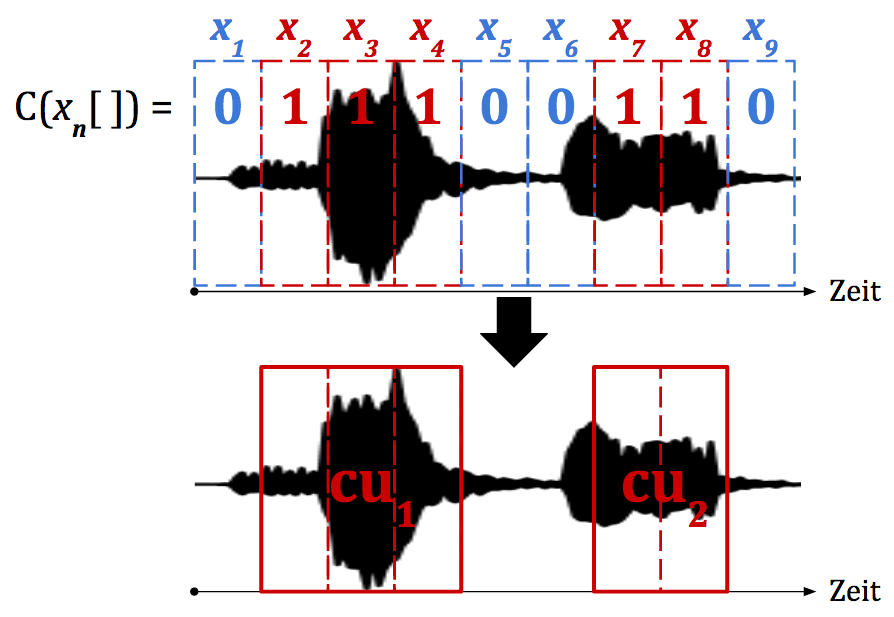
\includegraphics[width=0.6\textwidth]{bilder/cry-Unit02.png}
	\caption{Zusammenfassung der als stimmhaft klassifizierter Signalfenster zu Schreieinheiten}
	\label{img:cryUnit}
\end{figure}

\autoref{eq:cry-Unit} definiert den Datentyp \textbf{Schreieinheit} (engl. \emph{Cry-Unit}) [$CU$]. Eine Schreieinheit wird bestimmt durch einen Anfangszeitpunkt $start$, einen Endzeitpunkt $end$ und der Liste ihrer Signalfenster $windows = \big[x_0[\;], \ldots, x_n[\;]\big]$.

\begin{equation}
CU := \quad \Big(windows = \big[x_0[\;] \; ,\ldots, x_n[\;] \big] \;, start \in Zeit \;, end \in Zeit \Big)
\label{eq:cry-Unit}
\end{equation}

Die zeitliche Dauer eine Schreieinheit $cu \in CU$ wird nach \autoref{eq:cry-Lambda} berechnet und mit $\lambda$ bezeichnet. Die Dauer der Pause zwischen zwei Schreieinheiten d($cu_i, cu_j$), wird nach \autoref{eq:cry-distance} berechnet. Diese Zusammenhänge werden in \autoref{img:cryUnit-details} visualisiert.\cite[S. 2]{vad_entropy}

\begin{equation}
\lambda (cu) = cu.end - cu.start
\label{eq:cry-Lambda}
\end{equation}

\begin{equation}
\text{d}(cu_i, cu_j) = cu_j.start - cu_i.end
\label{eq:cry-distance}
\end{equation}

\begin{figure}[h]
	\centering
	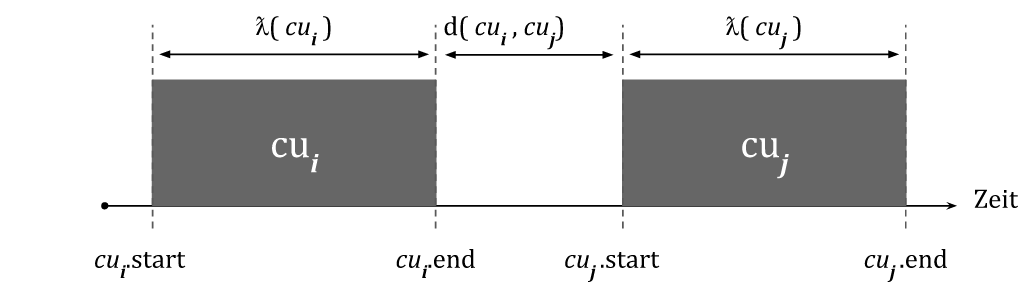
\includegraphics[width=0.95\textwidth]{bilder/newSmoothing05.png}
	\caption[Beziehungen zwischen benachbarten Schreieinheiten]{Beziehungen zwischen benachbarten Schreieinheiten (nach \cite[S. 2]{vad_entropy})}
	\label{img:cryUnit-details}
\end{figure}

Algorithmus \autoref{alg:cryUnit} zeigt in Pseudo-Code, wie in einem Eingangssignal $x[\;]$ die Schreieinheiten gekennzeichnet werden. Der Output des Algorithmus ist eine Liste aller im Signal detektierten Schreieinheiten $CU_{all} = [cu_0 , \ldots, cu_l]$. Die Funktion \textsc{turnSignalIntoOverlappingWindows} ($x[\;], length, hopsize$) zerlegt das Eingangssignal in einander überlappende Signalfenster. Wie in Unterabschnitt \ref{sec:windowing} beschrieben, wurde  $length = \SI{25}{\milli\second}$ und $hopsize = \SI{12.5}{\milli\second}$ festgelegt. Der Output dieser Funktion ist eine Liste aller Signalfenster $X_{all} = [x_0[\;] ,\ldots, x_m[\;]]$. Die Funktion $C(x_i[\;])$ ist diejenige, die im Zuge der Simulationsstudie der VAD festgelegt wurde und klassifiziert ein Signalfenster als \emph{Stimme} oder \emph{Sille} nach \autoref{eq:cepTree01}. Die Funktion \textsc{getTimeOf}$(x_i[\;])$ liefert den Anfangszeitpunkt des Signalfensters $x_i[\;]$. 

\begin{algorithm}[h]
	\caption{Detektion Schreieinheiten in einem Audiosignal}
	\label{alg:cryUnit}
	\begin{algorithmic}[1]
		\Function{DetectCryUnitsInSignal}{$x[\;], hopsize, overlap$}
		\State $X_{all} = $ \Call{turnSignalIntoOverlappingWindows}{$x[\;], hopsize, overlap$}
		\State $ CU_{all} \gets [\;]$
		\State $ cu\gets ([\;],0,0)$
		\For{\textbf{all} $x_i[\;] \in X_{all}$}
				\State $ c \gets C(x_i[\;])$
				\State \Comment Start of Cry-Unit
				\If {$c == 1 \wedge $ \Call{isEmpty}{cu.windows}}
						\State $cu\gets ([\;],0,0)$
						\State $cu.start \gets $ \Call{getTimeOf}{$x_i[\;]$}
						\State $cu.windows \gets [cu.windows, x_i[\;]]$
				\EndIf
				\State \Comment Inside Cry-Unit
				\If {$c == 1 \wedge $ \Call{isEmpty}{cu.windows}}
						\State $cu.windows \gets [cu.windows, x_i[\;]]$
				\EndIf
				\State \Comment End of Cry-Unit
				\If {$c == 0 \wedge $ ! \Call{isEmpty}{$cu.windows$}}
						\State $cu.end \gets $ \Call{getTimeOf}{$x_i[\;]$}
						\State $CU_{all} \gets [CU_{all}, cu]$
						\State $cu.windows \gets [\;]$
				\EndIf
		\EndFor
		
		%\State \Comment End last Cry-Unit by force if still open.
		%\If {$\text{ ! isEmpty}(cu.windows) == 0$}
		%\State $cu.end \gets  getTimeOf(X_{windows}[end])$
		%\State $CU_{all} \gets [CU_{all}, cu]$
		%\EndIf
		
		\Return $CU_{all}$
		
		\EndFunction
		
	\end{algorithmic}
\end{algorithm}


\section{Nachträgliche Korrektur von Schreieinheiten}
\label{sec:decision_smoothing_new}

\autoref{img:beforeSmoothing} zeigt ein Audiosignal mit einem Signal-Rausch-Abstand von \SI{5}{\decibel}, bei dem die Voice Activity Detection durchgeführt wurde. Die rote Linie zeigt die tatsächliche Klassifizierung und die grüne Linie die prognostizierte Klassifizierung. Es ist zu sehen, dass einige False-Negatives sowie False-Positives prognostiziert wurden. Es werden drei charakteristische Varianten falsch prognostizierter Klassifizierungen näher erläutert:

\begin{description}
	\item [False Negatives nach (a): ] Eine korrekt erkannte, längere Schreieinheit wird zu früh beendet. Oft werden kurz nach dem Ende einer längeren Schreieinheit sehr kurze Schreieinheiten prognostiziert, die eigentlich noch zu der längeren, vorhergehenden Schreieinheit gehören.
	\item [False Positives nach (b): ] Kurze Schreieinheiten werden in eigentlichen Stille-Bereichen erkannt.
	\item [False Negatives nach (c): ] Eine Schreieinheit zerfällt in zwei kürzere Schreieinheiten, da einige wenige Signalfenster in der Mitte als Stille erkannt wurden.
\end{description}

\begin{figure}[h]
	\centering
	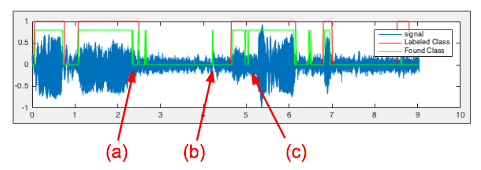
\includegraphics[width=0.8\textwidth]{bilder/smoothing02.png}
	\caption[Klassifizierung vor dem Decision-Smoothing]{Klassifizierung vor dem Decision-Smoothing}
	\label{img:beforeSmoothing}
\end{figure}

Im Process des \emph{Decision-Smoothing} werden kontextuelle Informationen genutzt, um nachträglich False-Positives und False-Negatives zu entfernen. Dazu werden die von Waheed et al. \cite{vad_entropy} präsentierten Ideen verwendet. Es werden zwei Parameter eingeführt: $\lambda_{min}$, die Mindestlänge einer akzeptierten Schreieinheit, und d$_{min}$, die Mindestlänge einer akzeptierten Pause zwischen Schreieinheiten. Das Decision-Smoothing wird nach den folgenden Entscheidungsregeln durchgeführt:

\textbf{Entscheidungsregeln: }\noindent\rule{0.7\linewidth}{0.3pt}
\begin{itemize}
	\item ist $\lambda (cu_{i}) \leq \lambda_{min}$ ?
	\begin{itemize}
		\item wenn $\lambda (cu_{i-1}) > \lambda_{min}$ und $d (cu_{i-1}, cu_{i}) \leq d_{min}$, dann vereinige $cu_{i}$ mit $cu_{i-1}$ $\Longrightarrow$ behebt False-Negatives des Types (a)
		\item ansonsten entferne $cu_i \Longrightarrow$ behebt False-Negatives des Types (b)
	\end{itemize}
	\item wenn $\lambda (cu_{i}) > \lambda_{min}$ und $d (cu_{i-1}, cu_{i}) \leq d_{min}$, dann vereinige $cu_{i}$ mit $cu_{i-1}$ . $\Longrightarrow$ behebt False-Negatives des Types (c)
\end{itemize}
\noindent\rule{\linewidth}{0.3pt}

Die Entscheidungsregeln greifen nur auf die letzten beiden erkannten Schreieinheiten zu, um eine kontinuierliche Analyse zu gewährleisten. Bei einer Offline-Analyse können die Entscheidungsregeln vereinfacht werden, da die False-Negatives nach Typ (a) und (c) mit der selben Regel abgefragt werden können. Algorithmus \autoref{alg:decisionSmoothing} zeigt in Pseudo-Code, wie das Decision-Smoothing durchgeführt wird. Input des Algorithmus ist eine Liste mit Schreieinheiten $CU_{all} = [cu_0 , \ldots , cu_l]$, die durch Algorithmus \ref{alg:cryUnit} entstanden ist, sowie die Grenzwerte $\lambda_{min}$ und $d_{min}$. Die Indexierung der Liste $CU_{all}$ beginnt bei 0. Der Output der Funktion ist eine Liste aller im Signal enthaltenenen Schreieinheiten $CU_{smoothed}$ mit korrigierten Anfangs- und Endzeitpunkten.
 
In verschiedenen Veröffentlichungen wurden unterschiedliche Mindestlängen von Schreieinheiten festgestellt. Várallyay \cite[S. 8]{cry_thesis} hat beispielsweise eine Mindestlänge von \SI{250}{\milli\second} gemessen. Der niedrigste Wert, der nach dem Wissen des Autors in einer Veröffentlichung genannt wurde, stammt von Zeskind et al. \cite[S. 325]{rythmic} und beträgt  \SI{60}{\milli\second}. Dieser Wert wurde für $\lambda_{min}$ in dieser Arbeit übernommen. Es konnten hingegen keine Veröffentlichungen gefunden werden, bei denen die geringste Pausenlänge gemessen wurde. Der Wert wurde ebenfalls mit $d_{min} = \SI{60}{\milli\second}$ bestimmt. \autoref{img:after-smoothing} zeigt das Beispielsignal vor und nach dem Decision-Smoothing. 

\begin{figure}[h]
	\centering
	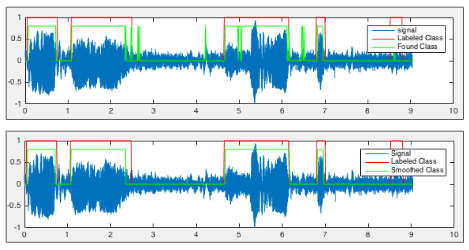
\includegraphics[width=0.8\textwidth]{bilder/smoothing04.png}
	\caption[Klassifizierung nach dem Decision-Smoothing]{Oben: Prognostizierte Klassifizierung vor dem Decision-Smoothing. Unten: Prognostizierte Klassifikation nach dem Decision-Smoothing.}
	\label{img:after-smoothing}
\end{figure}

\begin{algorithm}[h]
	\caption{Nachträgliche Korrektur von Schreieinheiten}
	\label{alg:decisionSmoothing}
	\begin{algorithmic}[1]
		\Function{decision-Smoothing}{$CU_{all}, \lambda_{min}, d_{min}$}
		\State $CU_{smoothed} \gets[CU_{all}[0]] $
		\State \Comment start for-loop at the \emph{second} cry-Unit!
		\For{ $i = 1 , \ldots ,$ \Call{length}{$CU_{all}$} - 1}
			\State $cu_i \gets CU_{all}[i]$
			\State $cu_{i-1} \gets CU_{smoothed}[end]$
			\If{$\lambda(cu_i) > \lambda_{min}$}
			\State \Comment Accept Cry-Unit
			\If{d$(cu_{i-1},cu_{i}) > d_{min}$}
					\State $CU_{smoothed} \gets [CU_{smoothed}, cu_i] $
			\Else
					\State \Comment Erase False-Negative of Type (c)
					\State $cu_i \gets $ \Call{vereinige}{$cu_i, cu_{i-1}$}
					\State $CU_{smoothed} \gets [CU_{smoothed}[1:end-1], cu_i] $
			\EndIf
			\Else
			\State \Comment Erase False-Negative of Type (a)
			\If{$d(cu_{i-1},cu_{i}) \leq d_{min}$ }
			\State $cu_i \gets $ \Call{vereinige}{$cu_i, cu_{i-1}$}
			\State $CU_{smoothed} \gets [CU_{smoothed}[0:end-1], cu_i] $
			\Else
			\State \Comment Don't accept $cu_i$. Erases False-Positives of Type (b)
			\EndIf
			\EndIf
		\EndFor
		
		\Return $CU_{smoothed}$
		\EndFunction
		
	\end{algorithmic}
\end{algorithm}




